\documentclass[a4paper,12pt]{article}
\usepackage[ukrainian,english]{babel}
\usepackage{ucs}
\usepackage[utf8]{inputenc}
\usepackage[T2A]{fontenc}
\usepackage{amsmath}
\usepackage{amsfonts}
\usepackage{graphicx}
\usepackage{wrapfig}
\usepackage{multirow}
\usepackage{flafter}
\usepackage{lscape}
\usepackage{rotating}
\usepackage{booktabs}
\usepackage{verbatim}
\newcommand\tab[1][1cm]{\hspace*{#1}}
\usepackage[left=20mm, top=20mm, right=10mm, bottom=20mm, nohead, nofoot]{geometry}
\usepackage{blindtext}
\begin{document}
\begin{titlepage}
\begin{center}
\large НАЦІОНАЛЬНИЙ ТЕХНІЧНИЙ УНІВЕРСИТЕТ УКРАЇНИ «КИЇВСЬКИЙ ПОЛІТЕХНІЧНИЙ ІНСТИТУТ» ФІЗИКО-ТЕХНІЧНИЙ ІНСТИТУТ	
\newline\newline\newline\newline\newline\newline\newline\newline\newline
\LARGE{ЛАБОРАТОРНА РОБОТА № 7\\
 ВИКОРІСТАННЯ ОБ'ЄКТНО-ОРІЄНТОВАНОГО ПІДХОДУ ДЛЯ РОЗРОБКИ ПРОГРАМНОГО ЗАБЕЗПЕЧЕННЯ}
\newline\newline\newline\newline\newline\newline\newline\newline\newline
\end{center}
\flushright 
Виконала:\\
студент групи  ФІ-12\\
Бекешева Анастасія \\

\end{titlepage}
\newpage
\tableofcontents
\newpage 
\section{Вступ}
Дана робота має задачу змоделювати космічний апарат. Її реалізація полягає в моделюванні структури космічного апарта, тобто з чого він скаладється та як працює. Проаналізувавши поставлену задачу, необхідно забезпечити в структурі космічного апарату: \begin{enumerate}
	\item Двигун
	\item Додаткові елменти, наприклад, сонячні панелі
	\item Головного за космічний апарат
	\item Персонал, розподілений за професіями
\end{enumerate}
У даній  роботі вище перераховані зауваження реалізовані введенням шести класів та встановленням певних відношень між ними.
\newpage
\section{UML-діаграма}
\includegraphics[width=17cm]{../labs/Spacecraft/Spacecraft}
\newpage\section{Код прогарми}\subsection{Main.swift}

\verbatiminput{../labs/Spacecraft/Spacecraft/main.swift}
\subsection{Spacecraft.swift}
\verbatiminput{../labs/Spacecraft/Spacecraft/Spacecraft.swift}
\subsection{Engine.swift}
\verbatiminput{../labs/Spacecraft/Spacecraft/Engine.swift}
\subsection{SolarPanels}
\verbatiminput{../labs/Spacecraft/Spacecraft/SolarPanels.swift}
\subsection{Personnel}
\verbatiminput{../labs/Spacecraft/Spacecraft/Personnel.swift}
\subsection{Scientist}
\verbatiminput{../labs/Spacecraft/Spacecraft/Scientist.swift}
\subsection{Engineer}
\verbatiminput{../labs/Spacecraft/Spacecraft/Engineer.swift}
\section{Скріни виконання роботи}
\begin{center}
	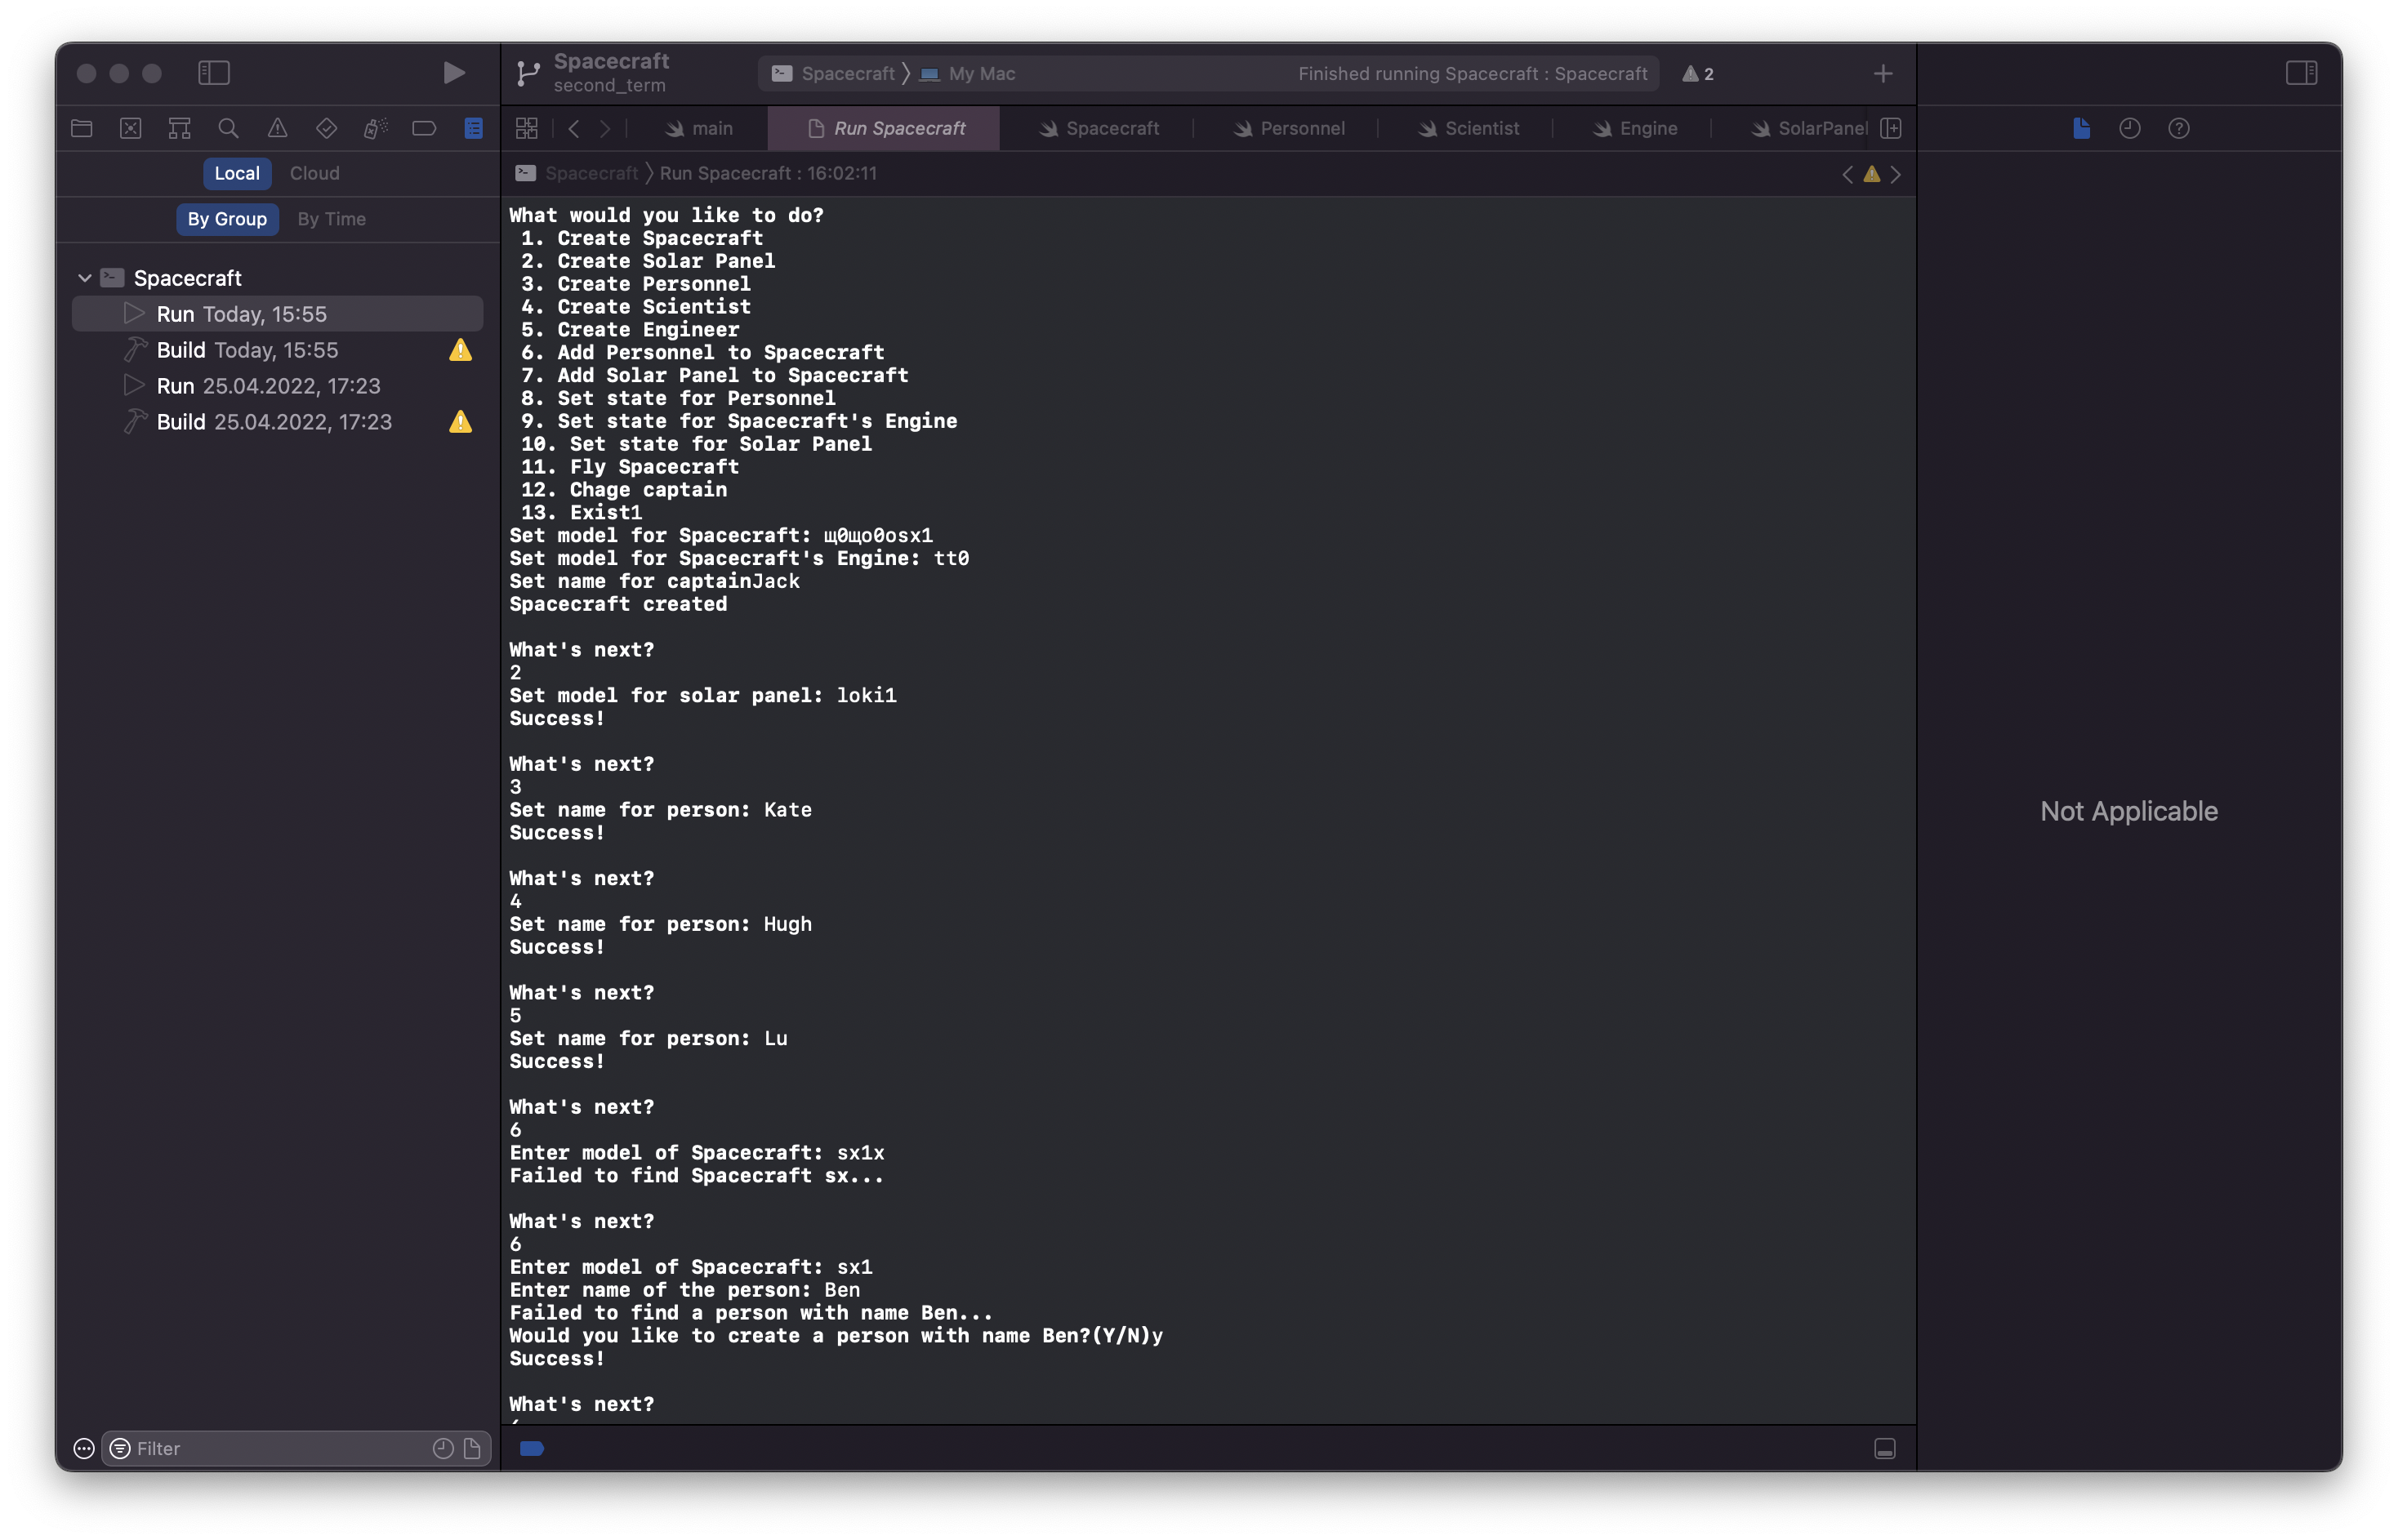
\includegraphics[width=18cm]{Screenshot1}\\
	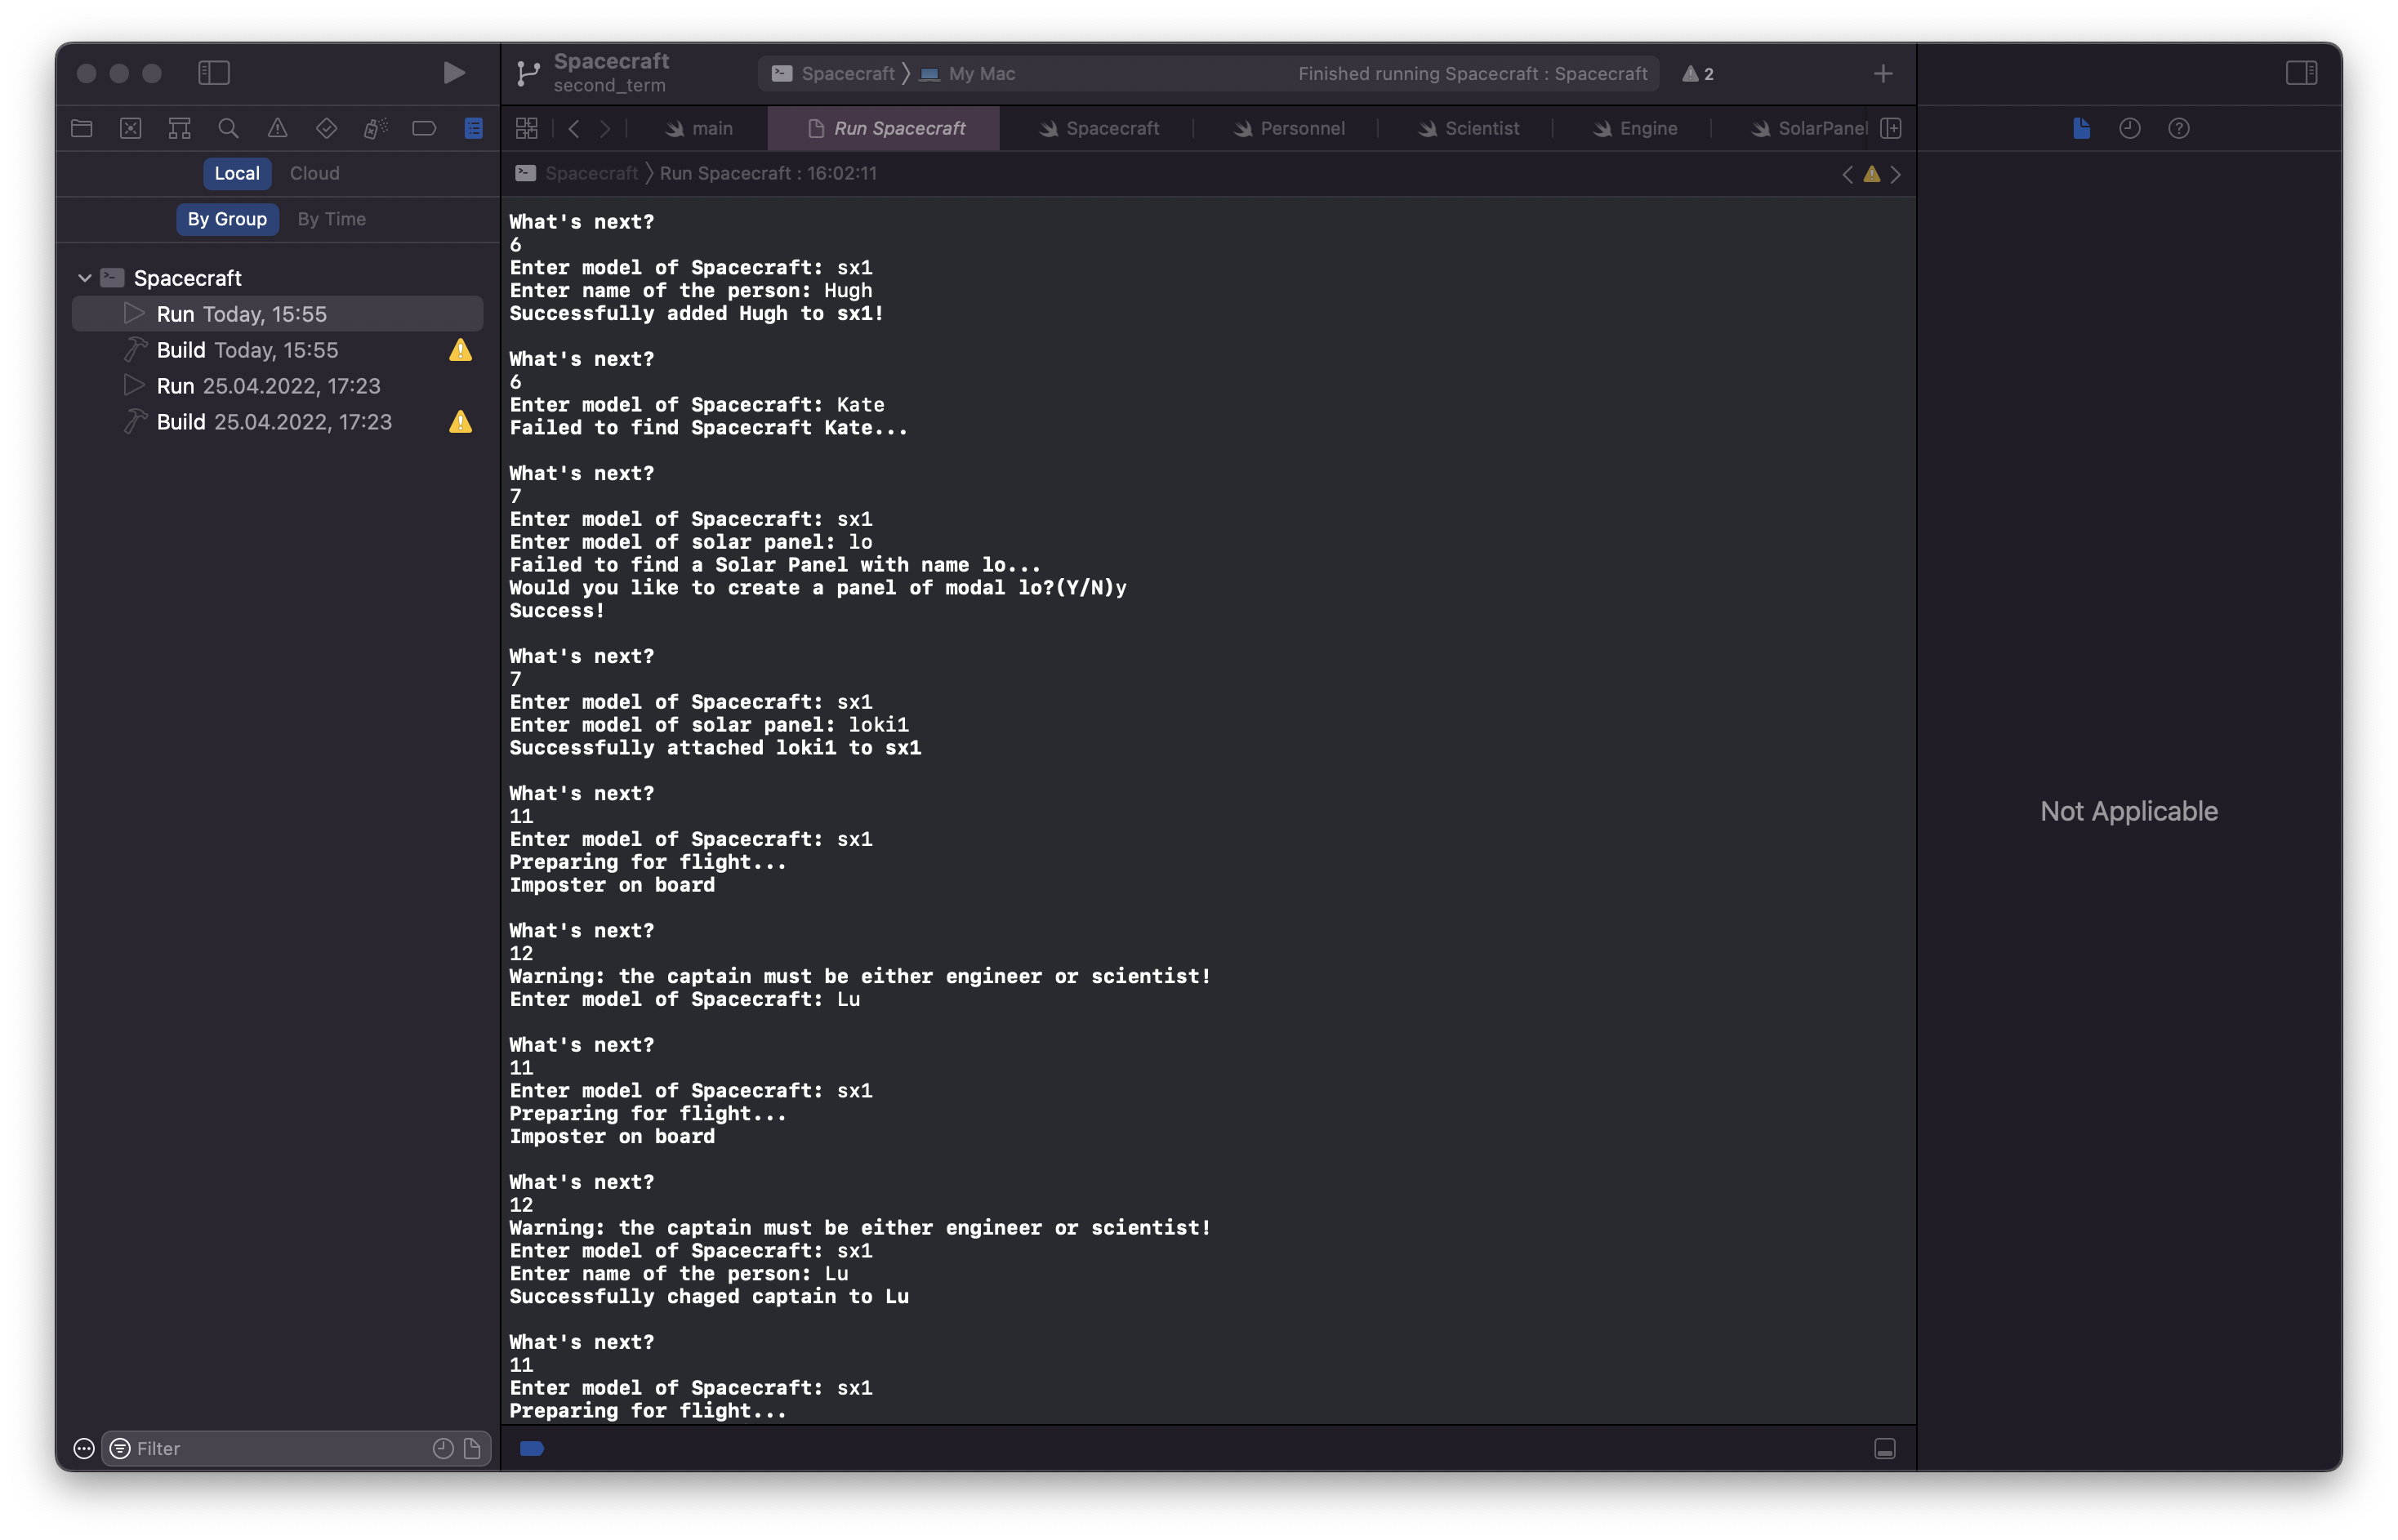
\includegraphics[width=18cm]{Screenshot2}\\
	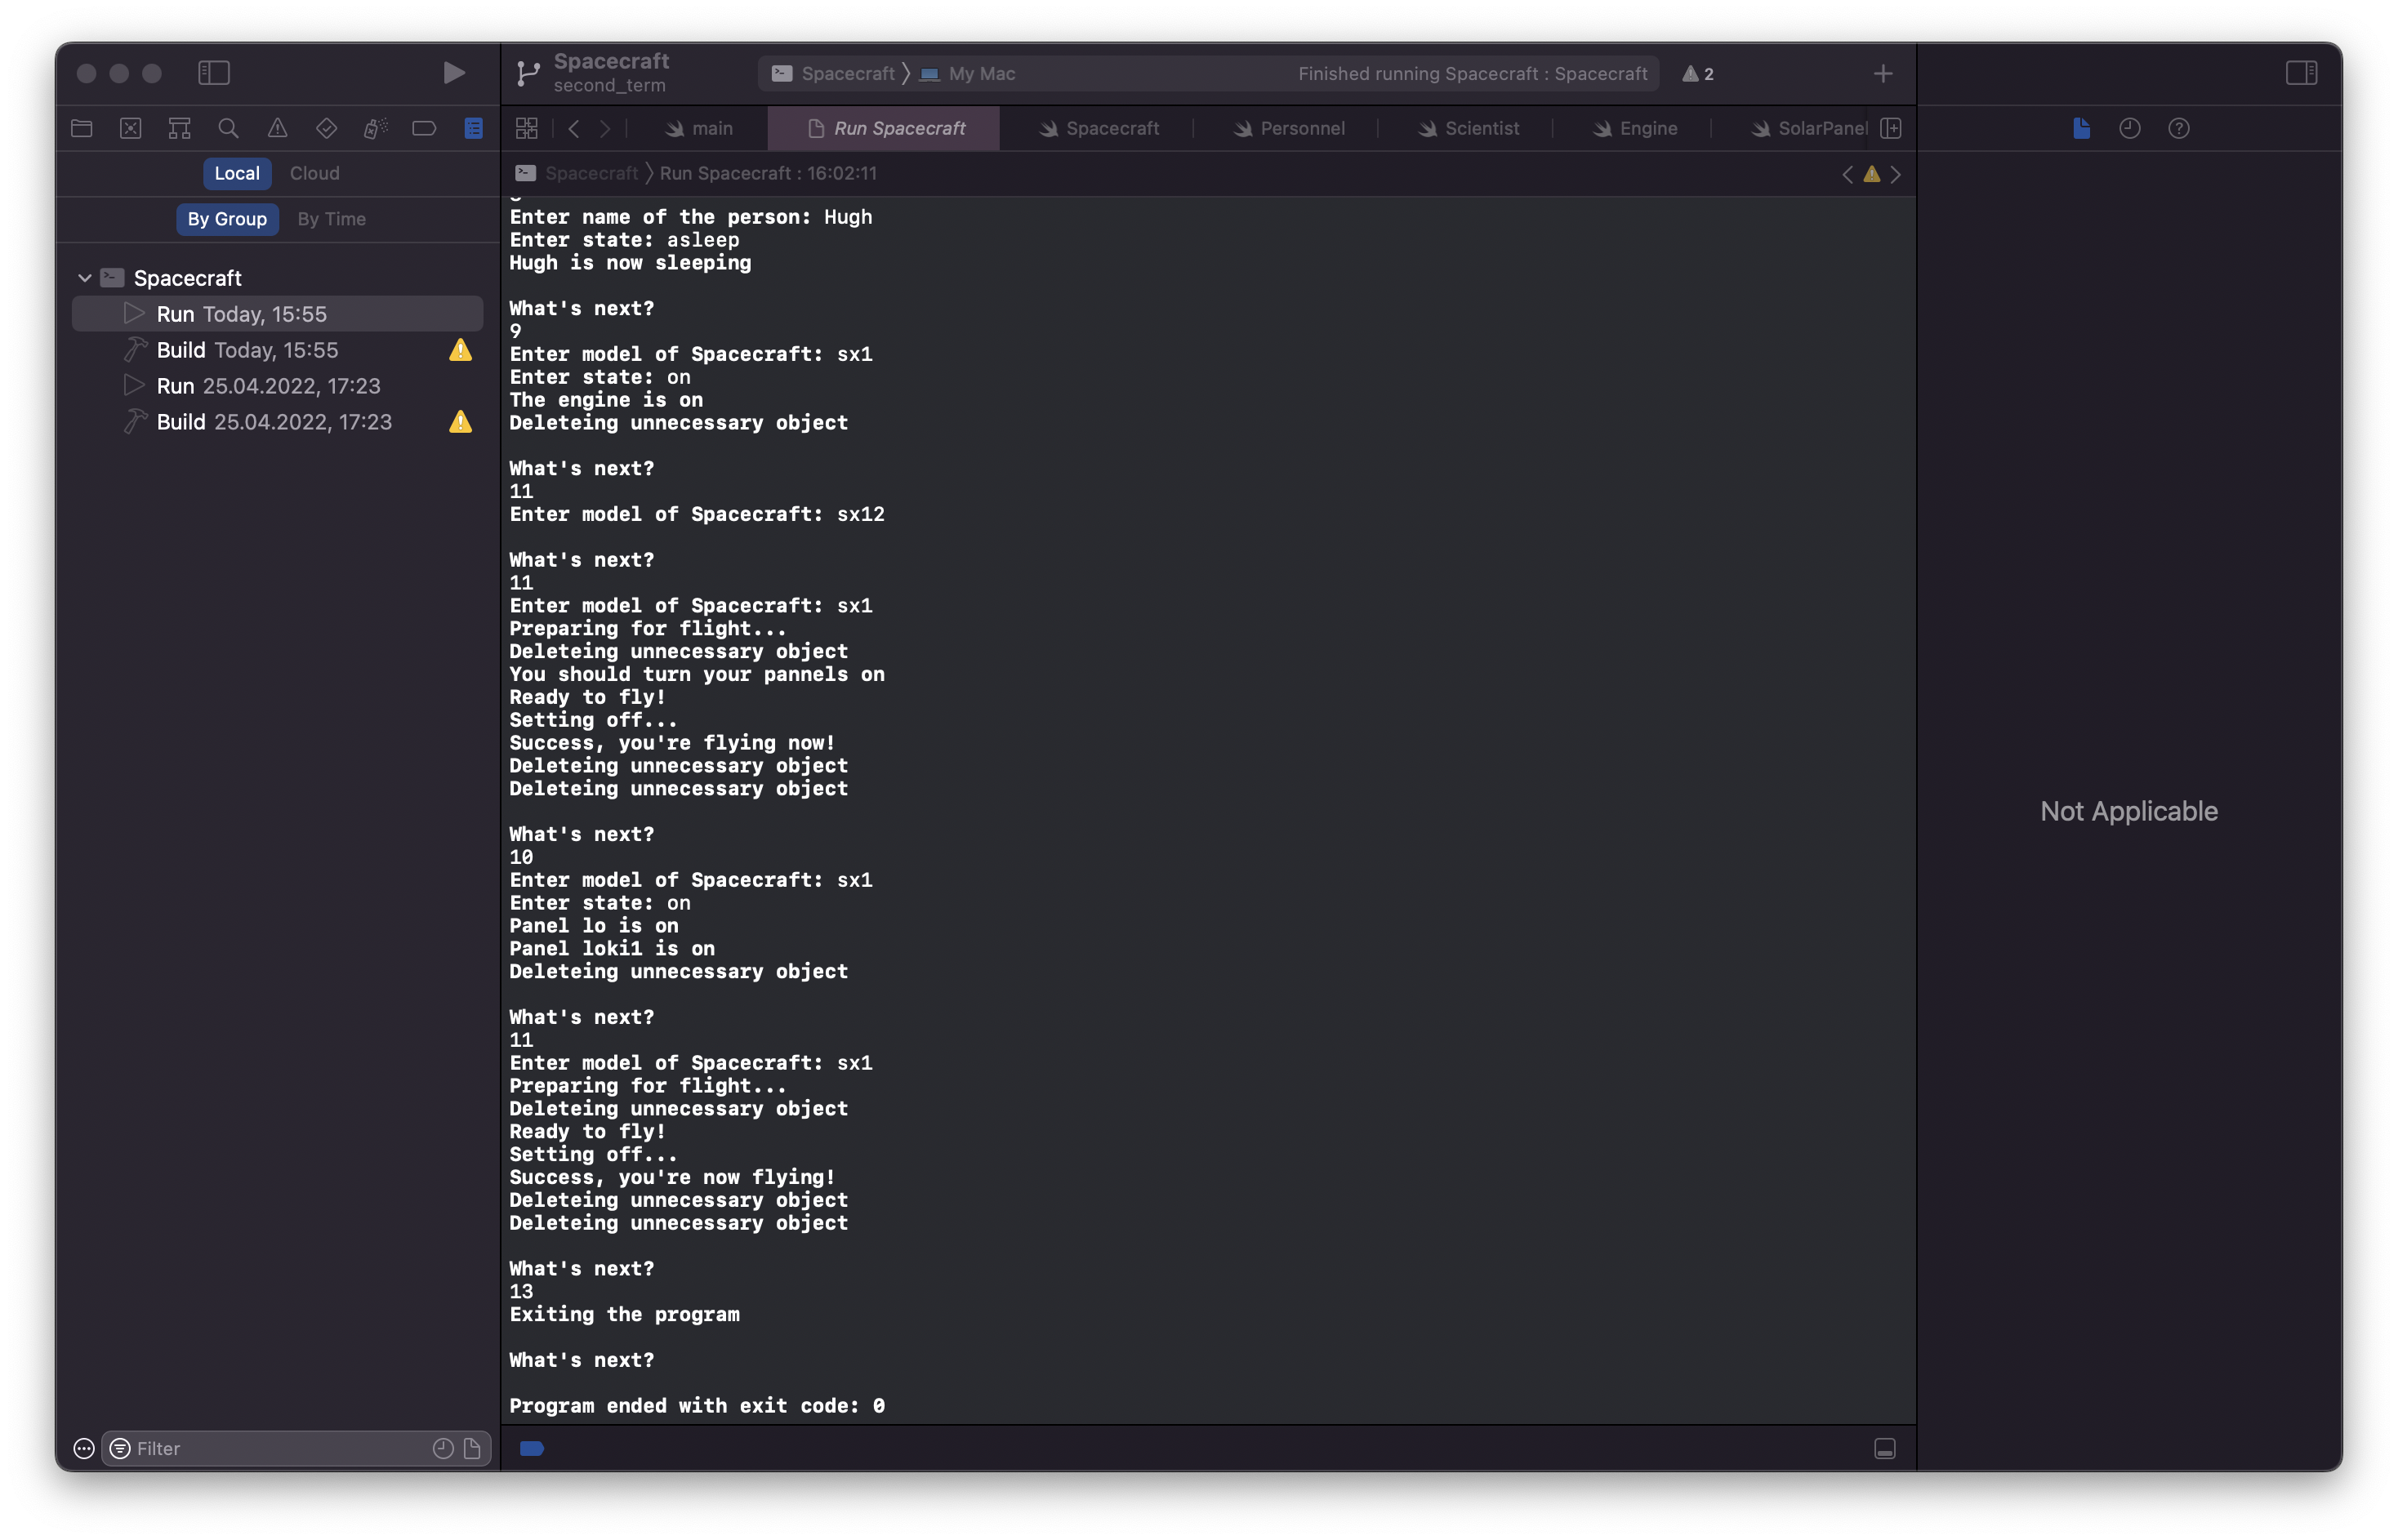
\includegraphics[width=18cm]{Screenshot3}
\end{center}









\end{document}